\begin{wrapfigure}{l}{0.4\textwidth}
    \vspace{-0.5cm}
    
\includegraphics[width=\linewidth]{intro/Recaptcha.png}
    
\includegraphics[width=\linewidth]{intro/Modern-captcha.jpg}
    \caption{ReCAPTHCA первой версии}
    \label{fig:ReCAPTHCAv1}
\end{wrapfigure}

Вы наверняка помните то время, когда интернет сайты постоянно заставляли вас разбирать, что написано на данных картинках. Сайты требовали это, чтобы избежать злоупотребления функционалом сайта со стороны ботов, предупреждая таким образом регистрацию множества "пользователей"\, отправку кучи сообщений или злоупотребления иным функционалом сайта или попытки перебора паролей.\\

Однако несколько лет назад вдруг подобные надписи пропали. Почему? Правоохранительные органы пересажали всех злоумышленников? Или они сами решили уйти в монастырь замаливать грехи. Вряд ли. Произошло то, что всегда происходит в таких случаях: всегда найдётся кто-то, кто захочет злоупотребить вашей системой во вред вам или во вред пользователям, ради кражи их данных, создания повышенной нагрузки на сервера и соответственно замедление или вообще прекращения их работы и других целей. Подобные люди никуда не делись и не денутся.\\

С появлением сайтов появились и скрипты, которые имитировали действия реальных пользователей, не являясь ими, создателям сайтов это не понравилось, поэтому они попытались отличить ботов от реальных пользователей. Первоначальной идеей было создать задание, с которым бы легко справлялись люди, но плохо справлялись роботы, такой задачей стала задача распознавания символов. Действительно для вас не составляет никакого труда разобрать, что значат все эти закорючки, линии и кружочки из которых состоят слова в этой книге (по крайней мере, я очень на это надеюсь). Но до недавних пор эта задача была для компьютеров совсем не тривиальной.\\

Так и появилось то, что называется капчей. Капча (от CAPTCHA — англ. Completely Automated Public Turing test to tell Computers and Humans Apart — полностью автоматизированный публичный тест Тьюринга для различения компьютеров и людей) — компьютерный тест, используемый для того, чтобы определить, кем является пользователь системы: человеком или компьютером. Термин появился в 2000 году. Основная идея теста: предложить пользователю такую задачу, которая с лёгкостью решается человеком, но крайне сложна и трудоёмка для компьютера. По состоянию на 2013 год, каждый день пользователями по всей планете вводится примерно 320 миллионов «капчей». \cite{wiki:captcha_def}\\

Но разумеется злоумышленники (и не обязательно злоумышленники, но и многие исследователи из научного интереса) не сдались и решили попытаться обойти защиту. Мы рассмотрим хронологию обхода ReCAPTCHA \-- пожалуй самую известную реализацию, изображение которой и было представлено выше, на \autoref{fig:ReCAPTHCAv1}.

\begin{itemize}
    \item 1 августа 2010 Chad Houck добился точности "взлома"\ капчи в 31.8\%.
    \item 26 мая 2012 Adam, C-P and Jeffball \-- 99.1\%. Следует уточнить, что ими была взломана аудио версия, при этом за несколько часов до презентации Google выпустил обновление  точность упала до 60.95\%.
    \item 27 июня 2012 - мексиканские студенты Claudia Cruz, Fernando Uceda, and Leobardo Reyes добились точности 82\%.
    \item Август 2017 - исследователи из университета Мериленда: Kevin Bock, Daven Patel, George Hughey, Dave Levin - 85.15\%.
\end{itemize}

Исследователи утверждали, что Гугл постоянно менял свою капчу, при этом часто возвращаясь к предыдущей версии\cite{wiki:captcha_is_hard}. Однако, всё же сложность капчи постепенно росла в конце концов требование, с которым она создавалась, --- быть сложной в решении для программ и лёгкой для людей, стало выполняться всё хуже. Так в августе 2012~--- более 90\% пользователей находят капчу сложной для ввода\cite{wiki:captcha_is_hard}. В мае 2016 была прекращена поддержка данного типа капчи, то есть она перестала обновляться, в 31 марта 2018 выключена окончательно.\cite{google:choose_recaptcha}\\

\begin{wrapfigure}{l}{0.4\textwidth}
    \vspace{-0.5cm}
    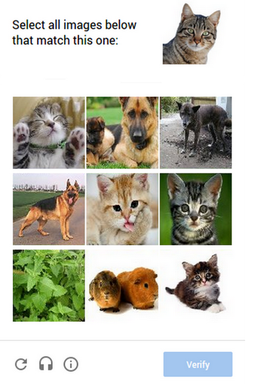
\includegraphics[width=\linewidth]{intro/recaptchav2.png}
    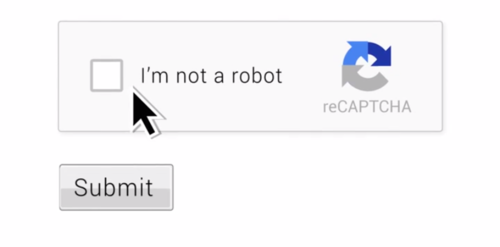
\includegraphics[width=\linewidth]{intro/recaptcha_I_am_not_a_robot.png}
    \caption{ReCAPTHCA второй версии}
\end{wrapfigure}

После этого гугл поменял тип своей капчи: теперь необходимо выбрать картинки с котиками, ибо все любят котиков. Таким образом гугл убивает сразу двух зайцев: отличает людей от ботов и создаёт обучающую выборку для своих алгоритмов распознавания текста и картинок. Перед этим была промежуточная версия, в которой выводилась фотография номера дома, соответственно пользователю нужно было разобрать этот номер, во славу google.maps.\\

Сейчас гугл развивает систему, которая анализирует действия пользователей: движения мыши, клики, нажатия клавиш. Люди не могут похвастать монотонностью действий, если боту нет смысла вести курсор прерывисто или не по прямой, нажимать клавиши с разной скоростью, а не середине ввода вообще отвлечься на звонок или сходить за чаем (в принципе, можно вообще не водить мышью или эмулировать физические нажатия клавиш, а использовать JS для совершения действий, но это уже совсем другая история). Разумеется создатели ботов тут же стали изменять свои алгоритмы, чтобы быть более человекоподобными (и автору самому приходилось этим заниматься), разумеется гугл тоже не стоит на месте, с каждым разом обходить защиту становится всё сложнее. Следует сказать, что эта капча, пожалуй, является самой дружелюбной к обычным пользователям, а мы ведь не хотим отпугивать пользователей необходимостью постоянно вводить свою электронную почту, sms коды подтверждения, и выбирать на каких картинках изображено что либо (кроме котиков, разумеется). Тут же человек сразу начинает пользоваться сайтом, скрипты в фоне анализируют его действия и их характер и в случае подозрения выводят уже обычную капчу или блокируют активность.\\

Как мы видим, алгоритмы машинного обучения заставили гугл постоянно менять свою систему, чтобы добиться необходимой эффективности защиты, во многом добиваясь этого использованием тех же алгоритмов: для того, чтобы распознавать, на какой именно части панорамы улицы находится номер улицы, и, следовательно, какую именно, часть следует отослать пользователям на проверку, и вывести метрики для отличия ботов от людей.\\

Рассмотрим ещё несколько сфер, в которых сейчас широко используется машинное обучение.\\\\

\textbf{Шахматы}\\
Пожалуй первой из популярных интеллектуальных игр, которые покорились машинному интеллекту, были шахматы.\\
\begin{itemize}
    \item В феврале 1996 года Гарри Каспаров победил шахматный суперкомпьютер Deep Blue со счетом 4-2. Этот матч выдающийся тем, что первую партию выиграл Deep Blue, автоматически став первым компьютером, победившим чемпиона мира по шахматам в турнирных условиях.
    \item В мае 1997 года Deep Blue II выигрывает матч у Гарри Каспарова со счётом $3\frac{1}{2}$ : $2\frac{1}{2}$.
    \item В 2000 году коммерческие шахматные программы Junior и Fritz смогли свести в ничью матчи против предыдущих мировых чемпионов Гарри Каспарова и Владимира Крамника.
    \item В ноябре-декабре 2006 года чемпион мира Владимир Крамник играл с программой DeepFritz. Матч закончился выигрышем машины со счётом 2-4.\\
\end{itemize}

Сейчас же даже у лучших гроссмейстеров нет шансов против среднего компьютера\cite{chess_human_has_no_chance}. При этом программы продолжают играть против друг друга и совершенствоваться в уровне игры и производительности алгоритмов.\\\\

\textbf{Го}\\
Шахматы пали перед алгоритмами и вычислительной мощью компьютеров, но многие годы считалось, что уж в других сферах компьютеры ещё долго не смогут составить конкуренцию человеку. Выражались мысли, что поле для игры слишком большое, что компьютер не сможет точно оценить текущую позицию, все возможные варианты её развития, выбрать оптимальный, у него просто не хватит на это "мозгов"\cite{go_is_hard}\cite{go_is_hard2}.\\

Конечно, доля правды в этих оценках была, притом немалая, однако, насчёт прогнозов, когда компьютеры смогут посоревноваться на равных с человеком, и причины, которые ему пока мешают были в корне неверными. В Го существует огромное количество возможных вариантов развития игры и позиций, для того, чтобы перебрать их все компьютеру потребуется время больше всей жизни вселенной, но ведь человек тоже не перебирает все возможные варианты, не делает этого и программа. Человек тоже весьма ограничен в своих способностях к оценке ситуации и вариантов её развития, не перебирает все возможности, выбирая лучшую, не делает этого и компьютер, для того, чтобы обойти человека не нужно играть идеально, нужно играть лишь лучше человека. На перебор всех вариантов шахмат тоже уйдёт время всей жизни вселенной, компьютер не перебирает все варианты в шахматах, не делает этого и в Го. Пожалуй, самой главной проблемой, препятствующей созданию эффективных алгоритмов,~--- являлось отсутствие хороших математических моделей, описывающих игру, с развитием и созданием этих моделей, появились и успехи у игровых программ:\\

\begin{itemize}
    \item В октябре 2015 года программа AlphaGo, разработанная компанией DeepMind выиграла у трехкратного чемпиона Европы Фань Хуэя (2 профессиональный дан) матч из пяти партий со счётом 4—1. Это первый в истории случай, когда компьютер выиграл в го у профессионала в равной игре.
    \item В марте 2016 года AlphaGo победила профессионала 9 дана Ли Седола в четырёх партиях из пяти.
    \item В мае 2017 года на саммите «Future of Go Summit» AlphaGo выиграла три партии из трёх в мини-матче с одним из сильнейших игроков в мире, лидером мирового рейтинга Эло Кэ Цзе.\\
\end{itemize}

Сейчас можно сказать, что все пошаговые настольные игры "сдались" программам, человек может победить в игре, только если правила были специально модифицированы правила, чтобы игроку было легче, или игра недостаточно заинтересовала исследователей, чтобы они разработали эффективные алгоритмы. Следующий шаг --- компьютерные игры в реальном времени. По числу своих возможностей и вариантов развития компьютерные игры, пожалуй, даже превышают настольные игры, однако, как мы выяснили, на примере шахмат и го, это лишь временное неудобство, а не принципиальная проблема, следующей ключевой особенностью является игра в реальном времени, в случае пошаговой игры, у компьютера (и у человека) есть время над обдумыванием хода вплоть до нескольких часов, в случае игры в реальном времени зачастую быстрое, но не оптимальное решение, лучше хорошего, но запоздавшего, а два решения лучше одного. Кроме этих проблем есть и другие, например, неполнота информации, в случае шахмат оба игрока видят всю доску и знают всю информацию об игре, однако, в компьютерные играх существует так называемый туман войны, который скрывает часть игровой карты, которая слишком далеко от существ или зданий игрока, таким образом, всегда приходится действовать в условиях неопределённости: вот в этом лесу, совсем рядом с твоей базой или персонажем уже могли затаиться враги, готовые атаковать, а могли и не затаиться, возможно, как раз таки наоборот, там небольшой разведывательный отряд, уничтожение которого, отбросит его назад.\\

И в этом направлении достигнуты реальные успехи, например, на International 2017 (август 2017) программная система побила одного из лучших игроков в мире Dendi в игре Dota 2 один-на-один\cite{dota:ai_vs_dendi}. И сейчас разрабатывается бот для игры пять-на-пять, в стандартном режиме для Dota 2\cite{dota:ai_vs_5}.\\

Другая команда в это время работает над ботом для компьютерной игры StarCraft\cite{starcraft:bot_vs_human}\cite{starcraft:bot_vs_human2}. Они обе используют одинаковую модель: бот просматривает повторы игр, анализирует кадры и стоит свою стратегию, во время игры используется модель обучения с подкреплением(reinforcement learning). Суть которой заключается в том, что бот принимает решения, а потом получает ответ от системы(игры), правильно он поступил или нет, и таким образом обучается.\\\\

\textbf{Распознавание номеров}\\
\begin{wrapfigure}{l}{0.4\textwidth}
    \vspace{-0.5cm}
    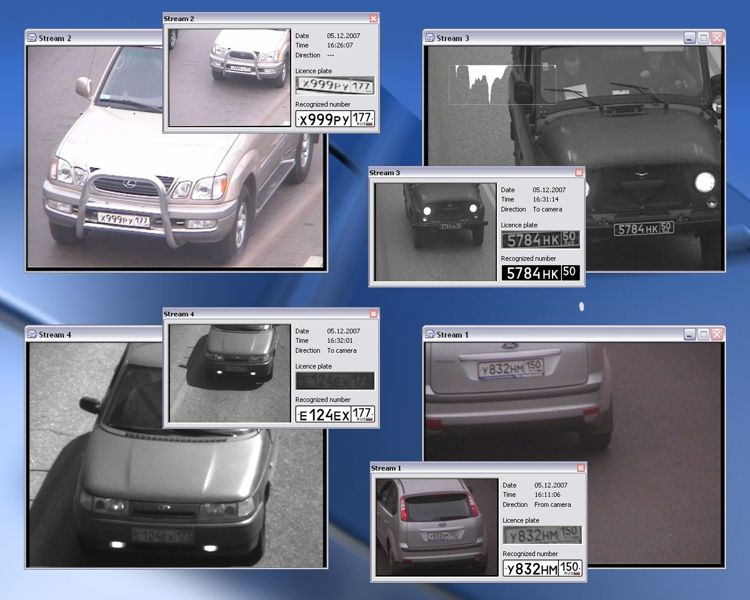
\includegraphics[width=\linewidth]{intro/numbers.jpg}
    \caption{Пример программы распознавания номеров}
\end{wrapfigure}






